\documentclass[twocolumns]{IEEEtran}
\usepackage{graphicx}
\usepackage{amsmath}
\usepackage{authblk}
\usepackage[english]{babel}
\usepackage{blindtext}
\usepackage[ruled,vlined,linesnumbered]{algorithm2e}
\usepackage{algorithmic,float}
\usepackage{setspace}
\usepackage{amsfonts}
\usepackage{hyperref}
\graphicspath{ {./images/} }
\usepackage{listings}
\usepackage[font=small,labelfont=bf]{caption}
\usepackage[table,xcdraw]{xcolor}
\usepackage[utf8]{inputenc}
\title{Parallelization of the Floyd-Warshall algorithm}
\author{David Bertoldi -- 735213 \\ email: d.bertoldi@campus.unimib.it}
\affil{Department of Informatics, Systems and Communication}
\affil{University of Milano-Bicocca}
\date{June 2020}
\begin{document}
\maketitle 
\begin{abstract}
The well known Floyd-Warshall (FW) algorithm solves the all-pairs shortest path problem on directed graphs. In this work we parallelize the FW using three different
programming environments, namely MPI, OpenMP and CUDA. We experimented with multiple data sizes, in order to gain insight on the execution behavior
of the parallelized algorithms on modern multicore and distributed platforms, and on the programmability of the aforementioned environments. We were able
to significantly accelerate FW performance utilizing the full capacity provided by the architectures used.
\end{abstract}
\section{Introduction and Background}
The FW is a classic dynamic programming algorithm that solves the \emph{all-pairs shortest path (APSP)} problem on directed weighted
graphs $G(V, E, w)$, where $V = \{1, \dots, n\}$ is a set of nodes, $E \subseteq V \times V$ are the edges and $w$ is a weight function $E \rightarrow  \mathbb{R}$
that expresses the cost of traversing two nodes. The number of nodes is denoted by $n$ and the number of edges by $m$ . \par
The output of the algorithm is typically in matrix form: the entry in the $i$th row and $j$th column is the weight of the shortest path between
nodes $i$ and $j$. FW runs in $\Theta(|V|^3)$ time and for this reason is a good choiche when working with dense graph: even though there
may be up to $\Omega(|E|^2)$ edges, the computational time is independent from the number of edges. \par
The FW algorithm is shown in Alg. \ref{alg:fw1}

\begin{algorithm}[h!]
\label{alg:fw1}
\SetAlgoLined

\For{$(u, v) \in E$}{
    $M_{u, v} \leftarrow w(u, v)$
}
\For{$v = 1 \rightarrow n$}{
    $M_{v, v} \leftarrow 0$
}
 \For{$k = 1 \rightarrow n$}{
  \For{$i = 1 \rightarrow n$}{
  \For{$j = 1 \rightarrow n$}{
  \If{$M_{i, j} > M_{i, k} + M_{k, j}$}{
 
    $M_{i, j} \leftarrow M_{i, k} + M_{k, j}$ 
 }
 }
 }
 }
 
 \caption[alg:fw1]{The Floyd-Warshall (FW) algorithm}
\end{algorithm}

A C implementation of this algorithm can be found \href{https://github.com/firaja/Parallel-FloydWarshall/blob/master/sequential.c}{here};
it is also referred in this document as \emph{sequential} implementation and it is used as base version when comparing to parallel implementations. \par \par



In particular we define the \emph{speedup} ($S$) of a given version $v$ of the algorithm as it follows:

\[S = \frac{T_{s}}{T_{v}}\]

where $T_v$ is the execution time of the version $v$ of FW and $T_s$ is the execution time of the \emph{sequential} version.

It is easy to notice that that the nested $i$ and $j$ for-loops are totally independent and therefore parallelizable.


\section{Parallel Programming Environments}

\section{Computational Platforms and Software Libraries}
\subsection{Sequential implementation}
The \emph{sequential} version of the FW algorithm can be found \href{https://github.com/firaja/Parallel-FloydWarshall/blob/master/sequential.c}{here}. In order to compile run
\begin{lstlisting}
$ gcc sequential.c -o sequential.out -O3
\end{lstlisting}
notice the \texttt{-O3} flag that makes the program run $3.5$ times faster.
\par
The \texttt{gcc} version used for this work is 7.5.0 and the program ran on a Intel Core i7-9700K. \\
Table \ref{tab:seq-time} shows the execution time (expressed in milliseconds) depending on the number of nodes
in the environment.


\begin{table}[h!]
\centering
\begin{tabular}{|l|l|}
\hline
\rowcolor[HTML]{3166FF} 
{\color[HTML]{FFFFFF} \textbf{Vertices}} & {\color[HTML]{FFFFFF} \textbf{Execution time (ms)}} \\ \hline
1000                                     & 1095                                                \\ \hline
2000                                     & 8860                                                \\ \hline
5000                                     & 138643                                              \\ \hline
7500                                     & 468750                                              \\ \hline
10000                                    & 1112111                                             \\ \hline
12500                                    & 2170138                                             \\ \hline
\end{tabular}
\caption{Execution time of the \emph{sequential} FW}                                                                                                                                            
\label{tab:seq-time} 
\end{table}

Figure \ref{fig:seq-time} shows the trend of the execution time. 

\begin{figure}[h!]
\centering                                                                        
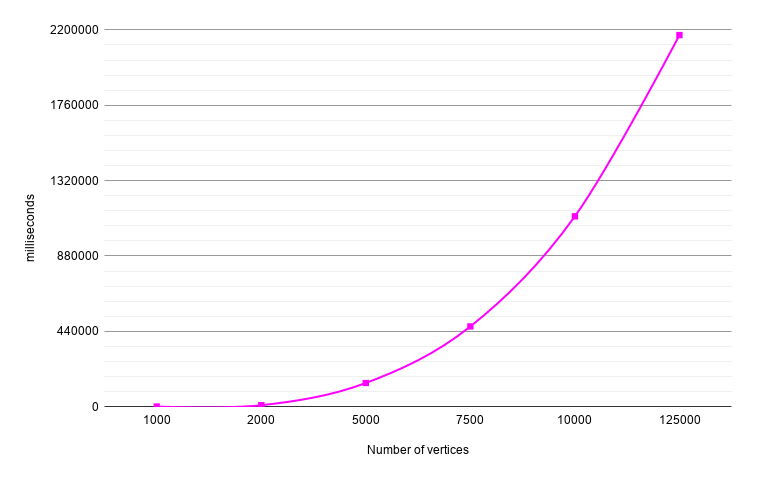
\includegraphics[width=3in]{images/seq-time}
\captionsetup{justification=centering,margin=2cm}                                                                                                                                   
\caption{Trend of the execution time based on Table \ref{tab:seq-time}}                                                                                                                                            
\label{fig:seq-time}                                                                                                                                                           
\end{figure}


It is easy to notice that the graph represent a 
third grade curve; this is the interpolated function starting from the collected data:
\[f(n) = 2.22n^3 - 18.83n^2 + 92.14n -94.84 \]



\subsection{MPI implementation}

The \emph{MPI} version of the FW algorithm can be found \href{https://github.com/firaja/Parallel-FloydWarshall/blob/master/mpi.c}{here}. In order to compile run
\begin{lstlisting}
$ mpicc -g -Wall mpi.c -o mpi.out -O3
\end{lstlisting}






\bibliographystyle{ieeetr}
\bibliography{Bibliography}
\end{document}